\part[Ablauf, Organisation und Umfeld]{Ablauf, Organisation und Umfeld
    }

\tableofcontents

\chapter{Aufgabenstellung}

\section{Titel der Arbeit}
Hitobito: Neue Generation von Personen-Filtern

\section{Ausgangslage}
Hitobito ist eine Open Source Webapplikation zum Verwalten von Mitgliedern, Events und vielem mehr. Die Ruby on Rails Applikation wurde 2012 von Puzzle ITC initiiert und wird stets weiterentwickelt.

Die Basis für die Software bildet das Webframework Ruby on Rails. Für das User Interface wird neben statischer Technologie wie HTML und CSS auch JavaScript oder Hotwire verwendet. Der komplette Source-Code steht auf Github zur Verfügung: \href{https://github.com/hitobito/}{Hitobito}

Eine Kernfunktionalität von Hitobito ist das Filtern von Personenlisten und von Mailinglistenempfängern mit konfigurierbaren Filtern. Diese werden über das Webinterface konfiguriert. Das Webinterface wurde mit statischen Web technologien entwickelt und ist inzwischen ziemlich in die Jahre gekommen.

Eine Erneuerung dieser Komponente ist ein Wunsch vieler Kunden.

\newpage

\section{Detaillierte Aufgabenstellung}
Mit dieser IPA soll ein neues UI mit Hotwire für die Persistierung von Filter-Parametern im Hitobito Generic-Wagon erstellt werden (rein Frontend).

\begin{itemize}
    \item Die Ansichten zur Konfiguration für Filter der Personenlisten und Abonnemente werden mit dem neuen UI ersetzt.
    \item Die neuen Ansichten werden nach einem gegebenen Mockup umgesetzt. Dieses Mockup wurde vom Kandidaten in Zusammenarbeit mit einem UX Experten erarbeitet und muss als Grundlage für die Ausarbeitung des Interfaces verwendet werden. Des weiteren muss das Interface auf das visuelle Design der existierenden Applikation abgestimmt sein.
    \item Das Backend darf nicht angepasst werden, das heisst das neue Interface verwendet die bestehenden Endpunkte und schickt die Daten im selben Format wie das alte Interface. Dies muss mit automatisierten Tests sichergestellt werden.
    \item Formular zur Konfiguration von Personen-Listen Filter: Das bestehende Formular muss ersetzt werden durch eine neue Implementation mit den in Mittel und Methoden definierten Web Technologien. Diese neue Umsetzung muss es erlauben, dynamisch weitere Filterkriterien hinzuzufügen im Gegensatz zur alten Implementation welche mit einem statischen Formular implementiert ist.
    \item Formular zur Konfiguration von Abo-Empfänger Filter: Das bestehende Formular besteht aus mehrerern Teilen, wovon im Rahmen der IPA nur der Teil für die Globalen Filterbedingungen angepasst werden muss. Wie bei den Personen-Listen Filter muss das Formular nun dynamisch implementiert werden. Die Formulare für die weiteren Filterbedingungen werden im Rahmen der IPA nicht angepasst. 
    \item Code der während dieser IPA entsteht soll auf ein privates Github Repo gepushed werden. Die VFs haben dabei stets Lese-Rechte.
    \item Die Konventionen des Ruby Style Guide, des Rails Style Guide und für Git Commit Messages müssen eingehalten werden (siehe Mittel und Methoden).
\end{itemize}

\newpage

Out of Scope - wird erst nach der IPA umgesetzt:

\begin{itemize}
    \item Filterung für Rollen, Gruppen, Events, People bei Abonnementen.
    \item Anpassungen der Ansicht in den anderen Wagons.
    \item Anpassungen der bisher bestehenden Tests in Hitobito welche die zu erweiternden Ansichten betreffen.
\end{itemize}

Weitere Anforderungen zu spezifischen Bewertunskriterien: 

\begin{itemize}
    \item G1: Dokumentation fachlicher und technischer Anforderungen: Die fachlichen und technischen Anforderungen müssen dokumentiert werden.
    \item G10: Konforme Implementierung und Versionierung: Applikationen und Schnittstellen müssen konform implementiert und versioniert werden.
    \item A13: Erhebung und Dokumentation der Bedürfnisse und Umfeld: Die Bedürfnisse und das Umfeld werden adäquat erhoben und dokumentiert.
    \item A15: Instruktion: Es wird für den Projektowner eine Instruktion durchgeführt. Diese muss dem Projektowner die relevanten Änderungen aufzeigen.
    \item C11: Einsatz von KI-Modellen: Wir setzen bei Puzzle KI in Form von Kopiloten und Chatbots als Hilfsmittel ein. Die Lernenden werden im sinnvollen Einsatz von solcher KI geschult. Dies umfasst z.B. den Umgang in Bezug auf Output Validierung, Transparenz und Sicherheit. Die IPA soll möglichst repräsentativ für unseren Alltag als Entwickler sein, dementsprechen darf KI ein Teil davon sein.
    \item G5: Risikoanalyse und Sicherheitsmassnahme: Sicherheitsrisiken von Applikationen und Schnittstellen müssen identifiziert und adressiert werden.
    \item G6: Entwicklung und Anpassung des Anforderungskatalogs: Ein Anforderungskatalog für Sicherheitsmassnahmen von Applikationen und/oder Schnittstellen muss erstellt oder angepasst werden.
    \item User Experience und visuelles Design: Das Feature muss visuell gut gestaltet sein um die Usability und Nutzerfreundlichkeit des Features sicherzustellen. 
    \item Versionsverwaltung mit Git (Source Code): Die Versionsverwaltung mit Git muss gemäss den Best Practices erfolgen. Es müssen sprechende und einheitliche Commit-Messages geschrieben werden und commit-spezifische Inhalte müssen passend zur Message sein und unter der Einhaltung der Firmenguidelines erfolgen. 
    \item Bewertung von Aussagen: Aussagen in der Arbeit müssen klar zwischen persönlichen Meinungen und auf Quellen basierenden Informationen differenziert werden.
\end{itemize}

\subsection{Mittel und Methoden}
Technologie und Plattform:

\begin{itemize}
    \item Ruby, Ruby on Rails, Active Record
    \item HTML, CSS, Javascript, Hotwire
    \item PostgreSQL
    \item Git
\end{itemize}

Entwicklungsumgebungen:

\begin{itemize}
    \item Intellij
    \item Visual Studio Code
    \item Github
    \item Rake
    \item Rubocop
\end{itemize}

Textverarbeitung und Diagramme

\begin{itemize}
    \item Latex
    \item draw.io
\end{itemize}

\subsection{Vorkenntnisse}
Marc arbeitet bereits seit einigen Monaten an Features von Hitobito. Ausserdem hat er bereits seit dem 2. Lehrjahr Erfahrung auch in anderen Ruby on Rails Projekten gesammelt.

\subsection{Vorarbeiten}
\begin{itemize}
    \item Vorbereitung Dokumentvorlage
    \item Probe-IPA: Vereinheitlichung der Personenlisten- und Abonnementenfilterlogik im Backend
    \item Entwurf eines Mockups
\end{itemize}

\subsection{Neue Lerninhalte}
\begin{itemize}
    \item Eigenständiges Umsetzen eines Designs nach gegebenem Mockup
    \item Eigenständiges Projektmanagement während der IPA
\end{itemize}

\subsection{Arbeiten in den letzten 6 Monaten}
\begin{itemize}
    \item Umsetzung diverser Features und Bugfixes für Hitobito (Ruby on Rails)
    \item Probe-IPA: Vereinheitlichung der Personenlisten- und Abonnementenfilterlogik
    \item PostgreSQL Migration Hitobito
    \item Ruby on Rails Major Upgrade Hitobito
\end{itemize}

\chapter{Firmenstandards}

\section{Code conventions}
Als Code convention werden die Ruby \href{https://github.com/rubocop/ruby-style-guide}{Style Guides} verwendet. 
Die Überprüfung dieser Style Guidelines wird mit Rubocop (Formatter) sichergestellt. Die Konfiguration
dieses Formatters ist unter \href{https://github.com/hitobito/hitobito/blob/master/.rubocop.yml}{rubocop.yml} ersichtlich.

\subsection{Mehrsprachigkeit}
Hitobito ist eine mehrsprachige Applikation. Alle Erweiterungen oder Anpassungen müssen
in Deutsch übersetzt werden. Übersetzungen werden in einer Übersetzungsdatei gespeichert oder können
vom Kunden in einem Tool namens Transifex verwaltet werden.

\subsection{Lizenz}
Hitobito ist ein Open Source Projekt.
In jedem File in Hitobito wird das Copyright für den jeweiligen Kunden in Kommentarform beschrieben. 
Diese Lizenz- und Kundeninformationen können über folgenden Befehl 
eingefügt werden:

\begin{verbatim}
    rake license:insert
\end{verbatim}

Die daraus entstehende Lizenz sieht wie folgt aus:

\begin{lstlisting}[language=Ruby]
    # Copyright (c) 2012 -2021 , hitobito AG . This file is part of
    # hitobito and licensed under the Affero General Public License version 3
    # or later . See the COPYING file at the top - level directory or at
    # https :// github . com / hitobito / hitobito .
\end{lstlisting}

\newpage

Alternativ dazu können diese Informationen mit 

\begin{verbatim}
    rake license:remove 
\end{verbatim}

entfernt oder mit 

\begin{verbatim}
    rake license:update 
\end{verbatim} aktualisiert werden.

\section{Git Commit Message Conventions}
Die Git Commit Messages werden nach den Regeln von Puzzle ITC formuliert. Im Anhang
unter \hyperref[sec:gitconv]{Git Commit Message Concention} finden sie eine Kopie der Firmenkonventionen. Diese wurden 
basierend auf folgendem Tutorial definiert: \href{https://cbea.ms/git-commit}{Tutorial}

\begin{itemize}
    \item Sprache: Englisch
    \item Kurze und prägnante Message, idealerweise unter 50 Zeichen
    \item Mit Grossbuchstaben beginnen
    \item Kein Punkt am Schluss
    \item Den \textit{imperative mood} (Befehlsform) verwenden, also «Fix bug with X» statt «Fixed bug with X» oder «More fixes for broken stuff»
    \item Wenn vorhanden Ticket referenzieren:
    \begin{itemize}
        \item Bei Open Project Work Packages: «Add X, refs \#12345»
        \item Bei Gitlab/Github Issues: «Add X \#12345»
    \end{itemize}
\end{itemize}

\chapter{IPA-Schutzbedarfanalyse}

\section{Datensicherheit}

\section{Applikationssicherheit}

\chapter{Organisation der IPA-Ergebnisse}
\section{Datensicherung}
In dieser IPA unterteilen wir die Datensicherung in:

\begin{itemize}
\item Dokumentation
\item Code
\end{itemize}

\subsection{Dokumentation}
\begin{table}[h!]
    \begin{tabular}{|L{0.4\textwidth}|L{0.5\textwidth}|}
        \hline
        \rowcolor{puzzleblue} \multicolumn{2}{|l|}{\color{white}\textbf{Dokumentation}} \\[12pt]
        \hline
        Tools & Git und USB \\
        \hline
        Versioniert & Ja \\
        \hline
        Interval & Mind. 2x täglich \\
        \hline
        Beschreibung & Die Dokumentation ist im ipa-puzzle-template Repository unter dem Branch probe-ipa angelegt.
        Sobald ein Dokumentationsticket abgeschlossen wurde, werden die Änderungen auf den Github Server in das private Repository
        gepushed. Dies geschieht mind. 2x täglich. Zusätzlich, wird pro Tag ein Ordner auf einem USB-Stick erstellt.  Am Ende des Tages wird eine Kopie der Dokumentation
        in diesen Ordner geladen. \\
      \hline
      \end{tabular}
      \caption{Sicherung Dokumentation}
\end{table}

\newpage

\subsection{Code}
\begin{table}[h!]
    \begin{tabular}{|L{0.4\textwidth}|L{0.5\textwidth}|}
        \hline
        \rowcolor{puzzleblue} \multicolumn{2}{|l|}{\color{white}\textbf{Code}} \\[12pt]
        \hline
        Tools & Git und USB \\
        \hline
        Versioniert & Ja \\
        \hline
        Interval & Mind. 2x täglich \\
        \hline
        Beschreibung & Für die Entwicklung wurden die Repositories hitobito und hitobito\-generic geforked.
        Auf diesen Repositories wird an Tagen an welchen entwickelt wird, mind. 2x täglich committed. An diesen Tagen
        wird zur doppelten Sicherung zusätzlich eine Kopie des Projektes auf den USB Stick gespeichert, unter dem Ordner des jeweiligen Tages. \\
      \hline
      \end{tabular}
      \caption{Sicherung Code}
\end{table}

% Nachweis Backup auf USB Stick %

\subsection{Wiederherstellung des Codes}
Im Falle eines Datenverlusts, können di Daten entweder über das Github Repository oder den USB-Stick wiederhergestellt werden.
Bei der Wiederherstellung mit Git wird der SSH-Key für die Klonung des Repositories benötigt. Ist
dieser SSH-Key nicht verfügbar, wird die Wiederherstellung über den USB-Stick vorgenommen und das Projekt des letzten Speicherstandes
kopiert. Im Falle des USB-Sticks ist mit mehr Datenverlust zu rechnen, falls der Datenverlust gegen Mittag oder Nachmittag auftritt, da
die Speicherung erst am Ende des Tages erfolgt. Aus diesem Grund ist die Datenwiederherstellung mit Git zu bevorzugen.

Die Nachweise für die jeweiligen Datensicherungen finden sie im Anhang.

\newpage

\section{Änderungskontrolle}
\begin{table}[h!]
    \begin{tabular}{|L{0.2\textwidth}|L{0.2\textwidth}|L{0.2\textwidth}|L{0.3\textwidth}|}
        \rowcolor{puzzleblue}\color{white}Version & \color{white} Datum & \color{white} Name & \color{white} Beschreibung \\
        \hline
        Vorlage & 27.02.2025 &  Marc Egli & Dokumentenvorlage \\
        \hline
        Version 0.1 & 04.03.2025 &  Marc Egli & Tag 1 abgeschlossen \\
        \hline
        Version 0.2 & 05.03.2025 &  Marc Egli & Tag 2 abgeschlossen \\
        \hline
        Version 0.3 & 06.03.2025 &  Marc Egli & Tag 3 abgeschlossen \\
        \hline
      \end{tabular}
      \caption{Änderungsprotokoll}
 \end{table}

\chapter{Projektmethode}
Die verwendete Projektmethode dieser IPA ist Scrum. Im folgenden Abschnitt wird der Einsatz, Abweichungen, Werkzeuge und Begründung der Wahl
dieser Projektmethode beschrieben. Des weiteren beschreibt dieser Abschnitt die Definition of Done (DoD).

\section{Einsatz von Scrum}

\subsection{Sprints}
Die IPA wird insgesamt in drei Sprints unterteilt. Jedem Sprint wird eine Phase der Arbeit zugewiesen. Die Aufteilung ist wie folgt:

\begin{itemize}
    \item Sprint 1: Initialisierung
    \item Sprint 2: Umsetzung
    \item Sprint 3: Finalisierung
\end{itemize}

\subsection{Verwaltungstool}
Als Verwaltungstool wird Github Projects eingesetzt. Das Board hierzu kann unter \href{https://github.com/users/Vakmeth/projects/3/views/1}{Github Board}
aufgerufen werden. Das Board ist in sechs Spalten unterteilt: 

\begin{itemize}
    \item Backlog: User-Stories werden grob erfasst, keine Details nötig.
    \item Refinement: User-Stories werden genauer Beschrieben und Akzeptanzkriterien werden definiert.
    \item Ready: User-Story wurde refined und geschätzt. Sie kann jetzt bearbeitet werden.
    \item In-Progress: User-Story wird momentan bearbeitet.
    \item In-Review: User-Story wurde abgeschlossen, alle Akzeptanzkriterien sind erfüllt.
    \item Done: User-Story erfüllt DoD (Definition of Done).
\end{itemize}

\begin{figure}[h]
    \centering
    \fbox{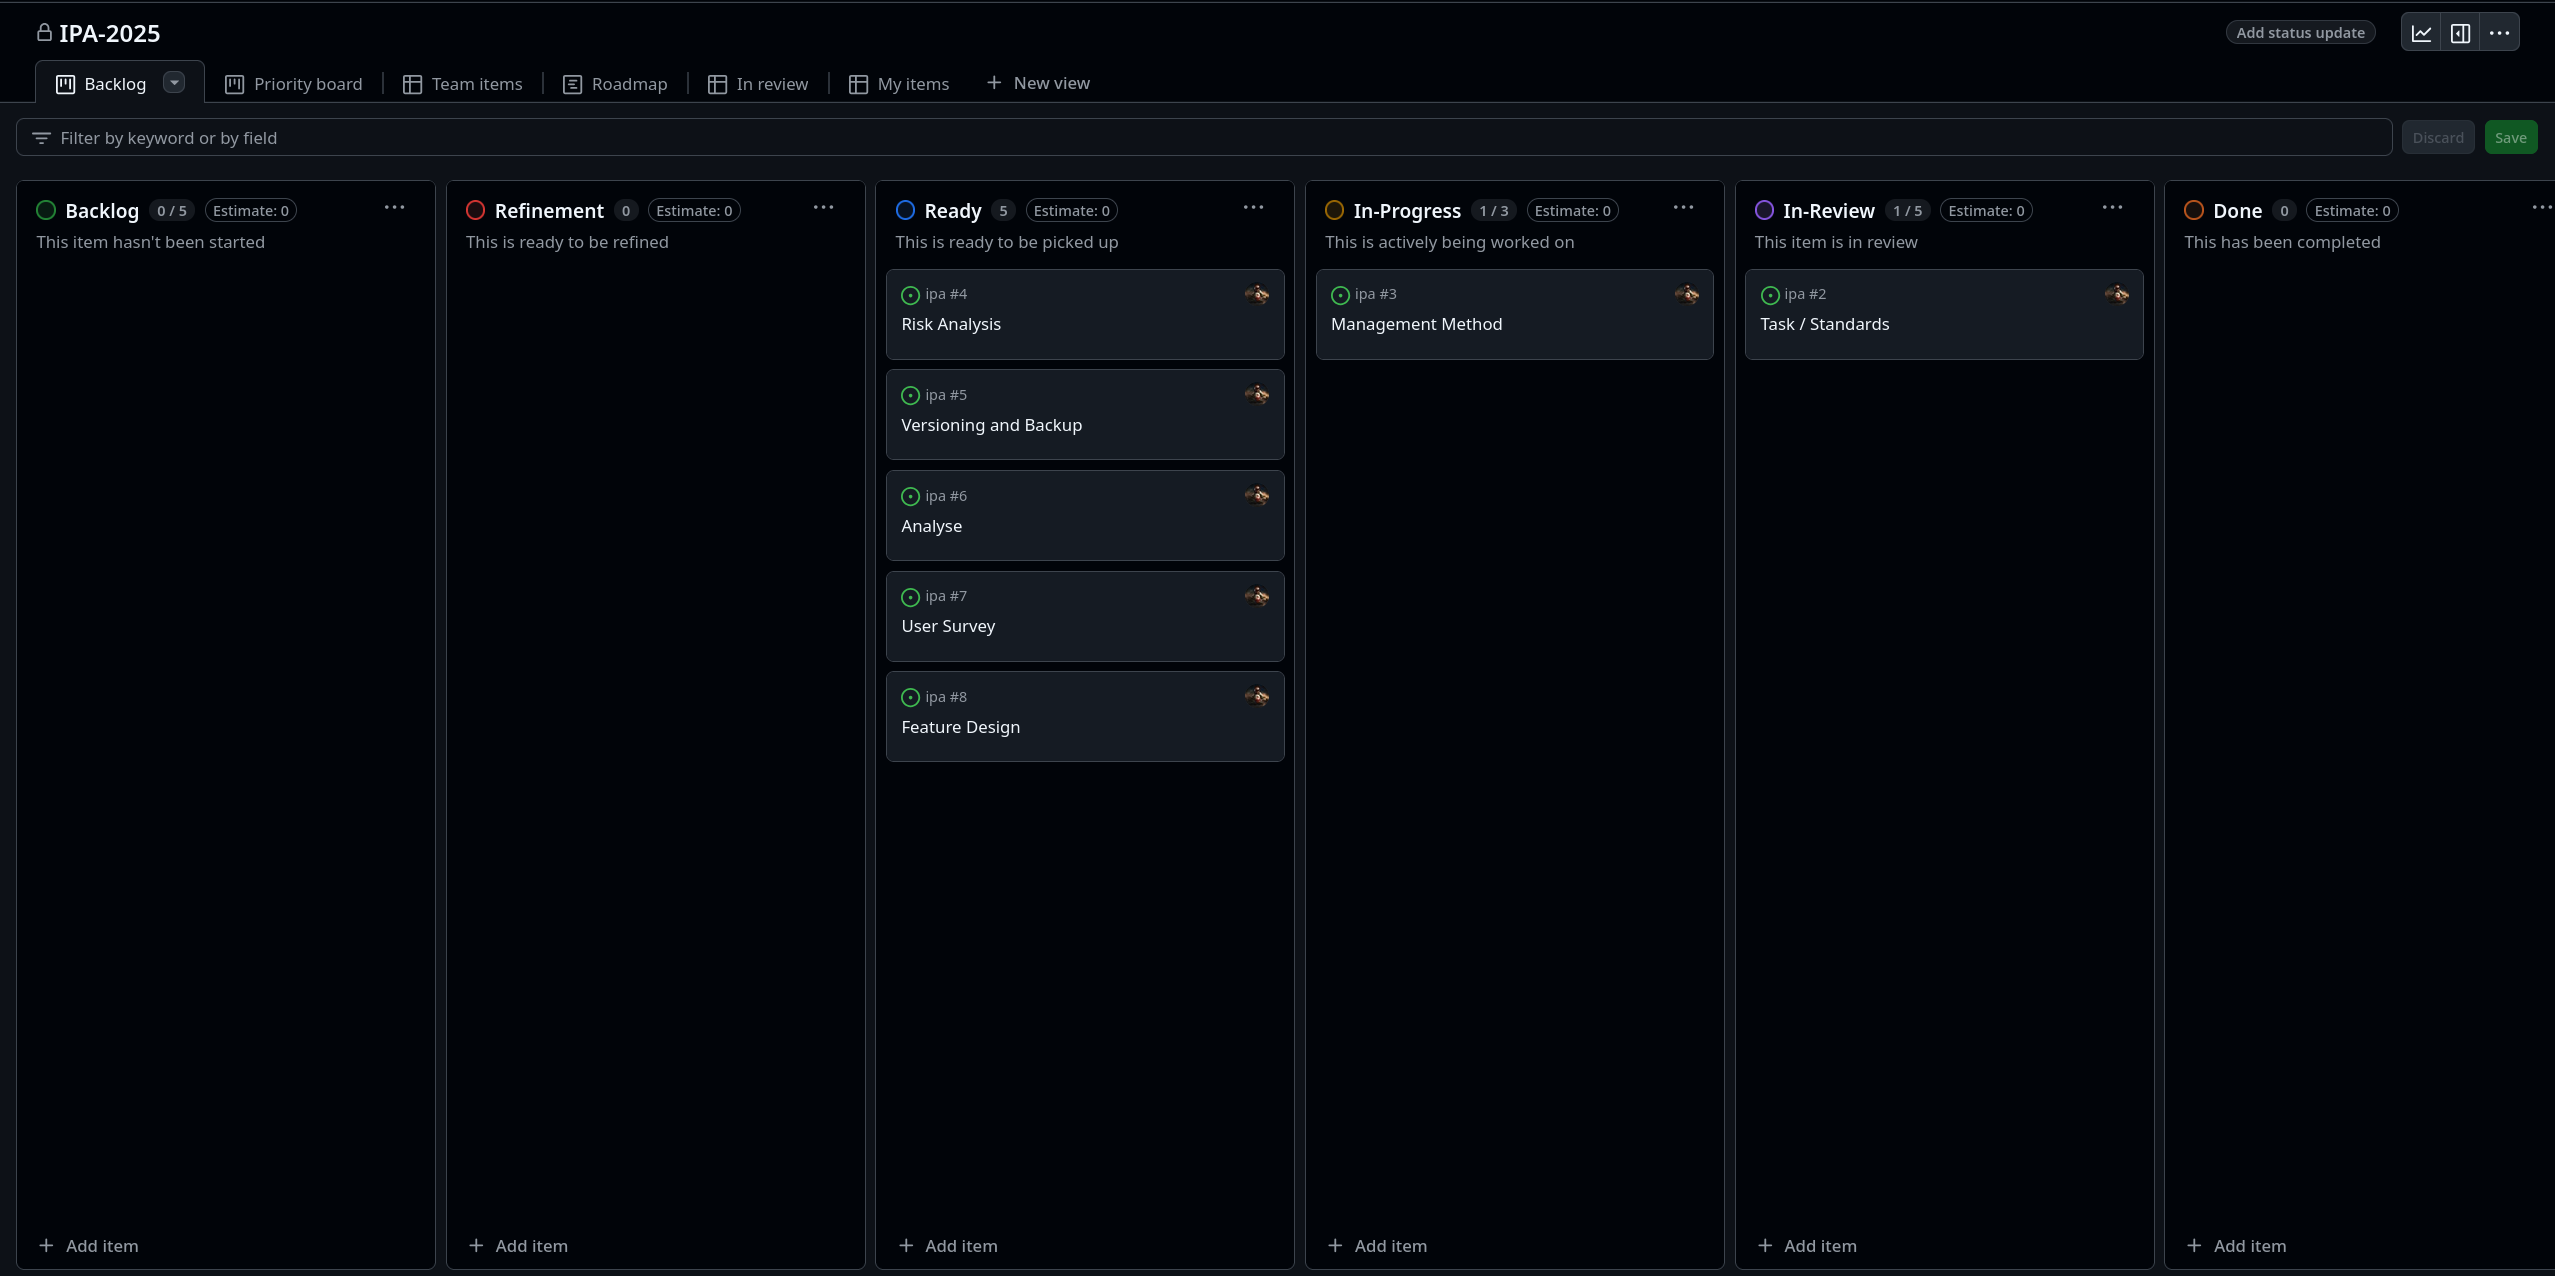
\includegraphics[width=1\textwidth,]{github_projects_board.png}}
    \caption{Github Projects Board}
\end{figure}

\subsection{Meetings}
\textbf{Sprint Planning}

Zu Beginn eines Sprints werden werden alle Aufgaben in Form von User-Stories im Backlog erfasst.
Die Stories werden anschliessend refined und danach geschätzt. Das Sprint Planning umfasst den Prozess der Erfassung
von User-Stories, deren Refinement und Schätzung. Konnten im letzten Sprint die geplanten User-Stories nicht alle abgeschlossen werden,
umfasst das Planning zusätzlich das Neurefinement und die Neuschätzung dieser User-Stories. Anwesend beim Sprint Planning ist auschliesslich
der Kandidat.

\textbf{Dailies}

Während eines Sprints wird jeden Tag um 09:00 Uhr ein Daily durchgeführt. Das Daily findet bei Puzzle ITC
im Sitzungszimmer "Sudo" statt. Anwesend sind dabei der Kandidat, die verantwortliche Fachkraft und die zusätzliche verantwortliche
Fachkraft. Ausgenommen von dieser Regel ist der erste Tag der IPA (04.03.2025) an welchem kein Daily durchgeführt wird. Grund dafür ist, dass zu diesem Zeitpunkt noch keine
Organisation und Projektvorgehensweise definiert wurde und die ersten Prozesse von Scrum erst ab dem 2. Tag eintreffen können.

Im Daily ist es dem Kandidat möglich, Fragen an seine verantwortlichen Fachkräfte zu stellen. Jedes Daily wird protokoliert. 
Die Protokolle der Dailies können unter \hyperref[sec:dailyprot]{Daily-Protokolle} eingesehen werden.

\textbf{Sprintabschlüsse}
\label{sprintfinish}

Nach jedem Sprint findet ein einstündiges Meeting für den Sprintabschluss statt. Darin werden die abgeschlossenen User-Stories
in der In-Review-Spalte verifiziert. Erfüllt die hinterlegte Arbeit alle Akzeptanzkriterien wird die User-Story auf Done geschoben. 
Sind die Akzeptanzkriterien nicht erfüllt, wird die User-Story auf Refinement geschoben. Anwesend beim Sprintabschluss ist auschliesslich der Kandidat.
In Folge des Sprintabschlusses wird das Sprint Planning durchgeführt.

\subsection{Abweichungen}
Trotz der Verwendung von Scrum, wurden Änderungen an der Definition dieser Projektvorgehensmethode
vorgenommen. Grund dafür ist, dass Scrum durch die Änderungen besser auf die IPA zugeschnitten ist.

\textbf{Schätzung}

Scrum verzichtet auf Schätzungen in Personenstunden und verwendet deswegen eine Währung namens "Story Points". Story Points werden
der \href{https://de.wikipedia.org/wiki/Fibonacci-Folge}{Fibonacci-Zahlenreihe} folgend vergeben. Der Sinn dabei ist, der Schätzung einer User-Story 
nach Personenstunden auszuweichen.

Dieses Konzept wird in dieser IPA verworfen, um in der Lage zu sein einen Zeitplan mit genauen Angaben in Personenstunden zu erstellen. Dies macht es dem Kandidaten
möglich besser einzuschätzen, wie gut er in der Zeit liegt.

\textbf{Abnahme Akzeptanzkriterien}

Nach Scrum werden User-Stories vom Product Owner abgenommen. Um ständige Meetings mit dem Product Owner von
Hitobito und den mithergehenden Zeitverlust zu vermeiden, werden die User-Stories vom Kandidaten selbt abgenommen. Den Prozess dazu
finden ist unter \hyperref[sec:sprintfinish]{Sprintabschlüsse} ersichtlich.

\newpage

\textbf{Sprint Retro}

Das Sprint Retro bietet dem Product Owner eine Möglichkeit einen Überlick über die Stimmung im Entwicklerteam zu erhalten. Sprint Retros finden 
im Geschäftsalltag Monatsweise statt. Auf das Sprint-Retro wird
in dieser Arbeit verzichtet. Grund ist der kleine Zeitrahmen der IPA, welcher es unnötig macht ein solches Meeting durchzuführen.

\section{Definition of Done}
\label{dod}
Die Definition of Done definiert wan eine User-Story abgeschlossen werden kann. Eine User-Story kann erst
abgeschlossen werden, wenn sie alle Kriterien der Definition of Done erfüllt. Im Rahmen der IPA werden zwei Definition of Done's verwendet.
Eine für User-Stories welche den Code betreffen, eine zweite für User-Stories welche die Dokumentation betreffen.

\subsection{DoD Code}

\begin{itemize}
    \item Nur notwendige Konsolenausgaben vorhanden
    \item Feature relevante Tests vorhanden
    \item Sprechender Code implementiert
    \item Nicht verwendete Methoden gelöscht
    \item Feature manuell getestet
    \item Alle Akzeptanzkriterien erfüllt
\end{itemize}

\subsection{DoD Dokumentation}

\begin{itemize}
    \item Definierte Sektion beschireben
    \item Kriterien aus Kriterienkatalog erfüllt
    \item Kriterien gemäss Dokumentenvorlage erfüllt
    \item Keine Grammatik- / Rechtschreibefehler vorhanden
    \item Quellen angegeben
\end{itemize}

\subsection{Akzeptanzkriterien}
Die Akzeptanzkriterien einer User-Story werden im dazugehörigen Ticket verwaltet. Jede User-Story wurde nach einem definierten Template
erstellt, welches in Github hinterlegt wurde. Eine User-Story kann folgendermassen aufgebaut sein:

\begin{figure}[h]
    \centering
    \fbox{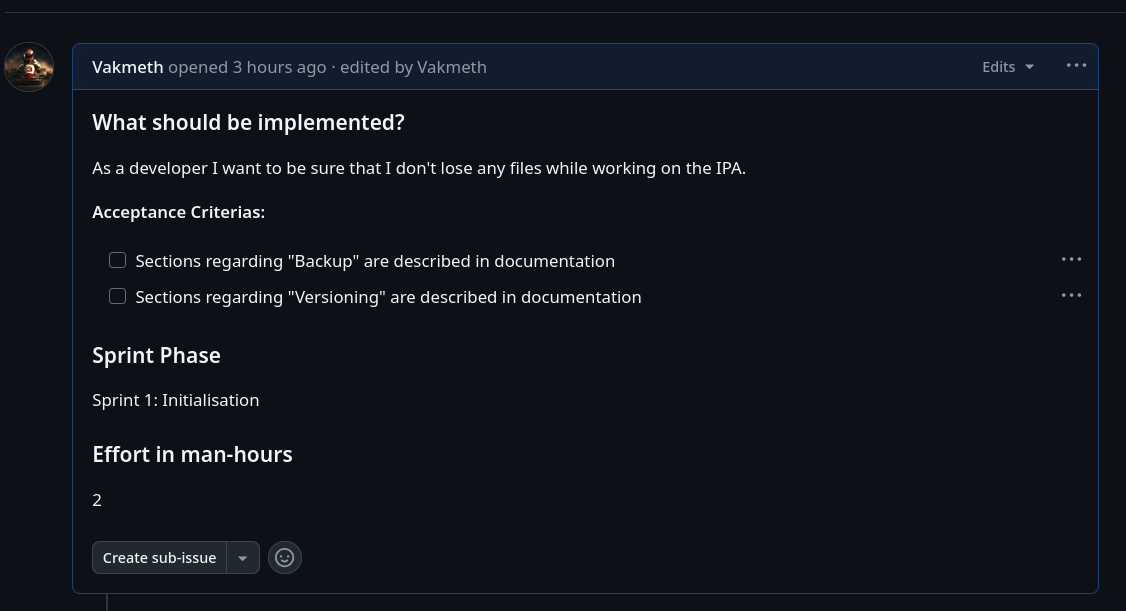
\includegraphics[width=0.8\textwidth,]{user_story.png}}
    \caption{Example of User Story}
\end{figure}

\section{Verwendungsgrund}
Die Projektvorgehensmethode wurde so gewählt, da sie für die IPA mehrere Vorteile bringt:

\begin{itemize}
    \item \textbf{Sprint Ende:} SCRUM zwingt den Entwickler dazu am Ende des Sprints ein vorzeigbares Produkt zu haben
    \item \textbf{Agilität:} Wenn eine Story nicht erreicht wurde, kann sie in den nächsten Sprint gezogen werden
    \item \textbf{Daily:} Durch die Dailies wird ein täglicher Austausch zwischen Fachkraft und Kandidat sichergestellt
    \item \textbf{Akzeptanzkriterien:} Mit den Kriterien verhindern wir das abschliessen von halbfertigen Features oder fehlerhafter Software
    \item \textbf{Board:} Durch das Github Projects Board ermöglichen wir eine schnelle Übersicht über den Stand der IPA
\end{itemize}

\chapter{Projektaufbauorganisation}

\section{Projektrollen Scrum}

\begin{figure}[h]
    \centering
    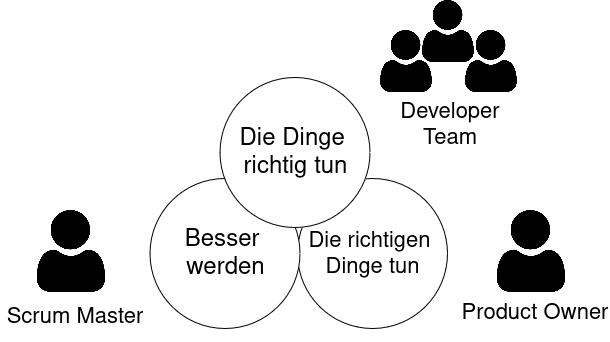
\includegraphics[width=1\textwidth,]{scrum_roles_ipa.png}
    \caption{Rollen in Scrum, selbstgezeichnet mit Draw.io}
\end{figure}

\begin{table}[h!]
    \begin{tabular}{|L{0.4\textwidth}|L{0.5\textwidth}|}
        \hline
        \rowcolor{puzzleblue} \multicolumn{2}{|l|}{\color{white}\textbf{Rollenbeschreibung}} \\[12pt]
        \hline
        Product Owner & Der Product Owner vertritt die Interessen des Kunden. Er priorisiert die Aufgaben im Product Backlog  \\
        \hline
        Scrum Master & Der Scrum Master unterstützt die Entwickler und beseitigt Hindernisse. Er sorgt für eine 
        kontinuierliche Verbesserung in der Arbeit. \\
        \hline
        Entwicklerteam & Das Entwicklerteam arbeitet selbstorganisiert den Sprint Backlog ab. 
        Durch Dailies wird ein laufender Informationsaustausch sichergestellt. \\
        \hline
      \end{tabular}
      \caption{Rollenbeschreibung}
\end{table}

\section{Projektrollen IPA}
\begin{table}[h!]
    \begin{tabular}{|L{0.4\textwidth}|L{0.5\textwidth}|}
        \hline
        \rowcolor{puzzleblue} \multicolumn{2}{|l|}{\color{white}\textbf{Rollenbeschreibung}} \\[12pt]
        \hline
        Verantwortliche Fachkraft & Unterstützt den Kandidaten von seiten des Lehrbetriebes. Erste Anlaufstelle bei Problemen.  \\
        \hline
        Zusätzliche verantwortliche Fachkraft & Unterstützung für die verantwortliche Fachkraft \\
        \hline
        Experten & \textbf{Validierungsexperte:} Validiert die IPA-Aufgabenstellung.
                    \textbf{Hauptexperte:} Verantwortlich für die Bewertung der IPA.
                    \textbf{Nebenexperte:} Unterstützung für den Hauptexperten. \\ 
        \hline
      \end{tabular}
      \caption{Rollenbeschreibung}
\end{table}

\newpage

\section{Projektrollen Scrum in der IPA}

\begin{figure}[h]
    \centering
    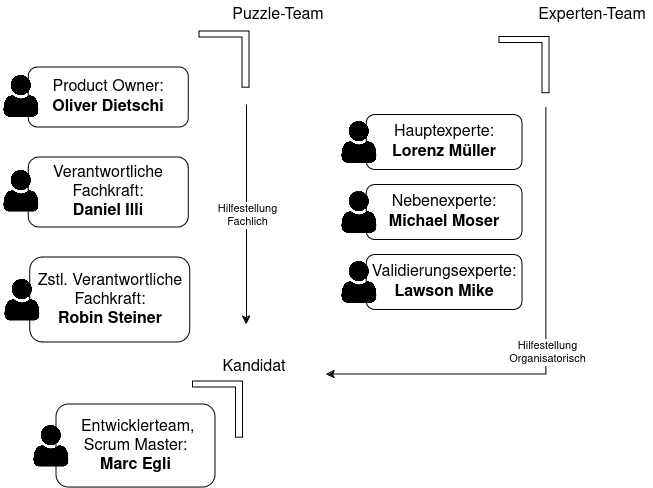
\includegraphics[width=1\textwidth,]{scrum_roles_division.png}
    \caption{Rollenverteilung in der IPA, selbstgezeichnet mit Draw.io}
\end{figure}

\begin{table}[h!]
    \begin{tabular}{|L{0.4\textwidth}|L{0.5\textwidth}|}
        \hline
        \rowcolor{puzzleblue} \multicolumn{2}{|l|}{\color{white}\textbf{Rollenbeschreibung IPA}} \\[12pt]
        \hline
        Verantwortliche Fachkraft & Daniel Illi  \\
        \hline
        Zusätzliche verantwortliche Fachkraft & Robin Steiner \\
        \hline
        Validierungsexperte & Lawson Mike \\ 
        \hline
        Hauptexperte & Lorenz Hess \\ 
        \hline
        Nebenexperte & Michael Moser \\ 
        \hline
        Scrum Master & Marc Egli \\ 
        \hline
        Development Team & Marc Egli \\ 
        \hline
        Kandidat & Marc Egli \\ 
        \hline
      \end{tabular}
      \caption{Rollenbeschreibung IPA}
\end{table}

\chapter{Zeitplan}

\section{Erläuterung zum Zeitplan}

\section{Sprints}

\newpage

\storeareas\zeitplan
\KOMAoptions{paper=a3, paper=landscape, DIV=current}
\areaset
  {\dimexpr\the\paperwidth-1cm\relax}% calculate requiered \textwidth
  {\dimexpr\the\paperheight-5.5cm\relax}% calculate requiered \textheight
\recalctypearea

% Figure %

\restoregeometry
\zeitplan
\newpage



\chapter{Arbeitsjournale}
\section{Tag 1: 04.03.2025}
\begin{table}[H]
    \begin{tabular}{|L{0.4\textwidth}|C{60pt}|C{60pt}|C{60pt}|}
        \hline
        \rowcolor{puzzleblue}\color{white}Tätigkeiten & \color{white}Beteiligte \color{white}Personen & \color{white}Aufwand Geplant (std) & \color{white}Aufwand Effektiv (std) \\
        \hline
         Raum einrichten, Kriterien aufhängen & Marc Egli & 1 & 1 \\
        \hline
        Zeitplan erstellen & Marc Egli & 1 & 1 \\
        \hline
        Sprint Planning & Marc Egli & 1 & 1.5 \\
        \hline
        Task / Standards beschreiben & Marc Egli & 1 & 1 \\
        \hline
        Management Method beschreiben & Marc Egli & 2 & 1.5 \\
        \hline
        Risikoanalyse beschreiben & Marc Egli & 2 & 2.75 \\
        \hline
        Arbeitsjournal schreiben & Marc Egli & 1 & 0.5 \\
        \hline
        \textbf{Total} &  & 8.25 & 9.25 \\
        \hline
    \end{tabular}
    \caption{Tätigkeiten Tag 1}
\end{table}

\subsection*{Tagesablauf}
Ich startet heute morgen um 07.45 Uhr mit der IPA. Als erstes begann ich damit, den Raum einzurichten, was bedeutet: 
Dockingstation anschliessen, Wasser bereitlegen und alle Kriterien meiner IPA aufhängen. Danach habe ich alle Kriterien mit verschiedenen
Farben unterteilt: Blau steht für Kriterien, welche über die gesamte IPA hinweg zählen, Rosa für Kriterien welche in der Umsetzung zu beachten sind und 
Gelb für Kriterien welche die Dokumentation betreffen. Als ich mit der Zimmereinrichtung fertig war, startete ich direkt mit dem Zeitplan. Ich passte das Template,
welches ich vorbereitet habe, auf die Dauer der IPA an und machte alles bereit um die ersen User-Stories einzutragen.  Nachdem der Zeitplan fertig war, startet ich das Sprint Planning.
Darin organisierte ich als erstes das Daily mit meiner verantwortlichen Fachkraft und meiner zusätzlichen verantwortlichen Fachkraft. Das Daily setzte ich auf
09:00 Uhr morgens an. 

Später im Planning habe ich alle nötigen User Stories für den kommenden Sprint definiert und diese anschliessend in den Zeitplan mit der dazugehörigen Schätzung übertragen.
Auf der Uhr war nun schon 11:15 Uhr. Ich startete den ersten Teil des Beschriebes der Aufgabenstellung und der Firmenstandards und ging danach in den Mittag.

Nach dem Mittag beendete ich den Beschrieb der Aufgabenstellung und der Firmenstandards und begann mit der Projektvorgehensmethode. Hier kam ich überraschend schnell durch und konnte so
nach 1.5 Stunden die Risikoanalyse beginnen an welcher ich bis kurz vor dem Schluss des Tages, 17:30 gearbeitet habe. Beim erstellen der Risikoanalyse, bemerkte ich, dass ich noch Fragen
zum Berechtigungskonzept in Hitobito hatte. Dementsprechend ging ich zu Niklas Jäggi, da er gerade zu gegen war, welcher mir dann das Konzept erklärte.
Ganz am Ende schrieb ich dann noch das Arbeitsjournal.

\subsection*{Hilfestellungen}
\begin{itemize}
    \item Niklas Jäggi: Erklärung des Berechtigungsaufbaus in Hitobito
\end{itemize}

\subsection*{Reflexion}

\subsubsection*{Was lief gut}
Der Einstieg lief meiner Meinung nach sehr gut. Ich kam schnell voran und konnte die ersten paar Teile der Dokumentation
beschreiben. Sogar das erste Kriterium, A11 (Projektaufbauorganisation) konnte ich scho abschliessen, was mich sehr motiviert hat. 

\subsubsection*{Was lief weniger gut}
Obwohl ich schnell voran kam, habe ich heute dennoch den geplanten Aufwand um 1/4-Stunde überschossen. Hier muss ich aufpassen, dass ich unbedingt früher anfange das
Arbeitsjournal zu schreiben. Zusätzlich hatte ich beim Sprint Planning ein Problem mit dem Erstellen eines Issue-Templates. Ich hatte mich spontan dazu entschieden,
dass es sehr hilfreich wäre, ein Template zu haben, in welchem man neue Issues während der IPA erfassen kann und so nicht alles immer neu machen muss. Allerdings hatte ich noch 
nie ein solches Template erstellt, wesegen das Planning dann auch eine 1/2-Stunde mehr Zeit in Anspruch nahm als geplant.

\subsubsection*{Meine Erkenntnisse von heute}
Nicht zu viel Zeit mit Themen verlieren, in welchen ich wenig Erfahrung habe. Besser wäre es gewesen mit dem Issue-Template
und dann in einem Daily danach zu fragen. Dennoch kann ich nun das Wissen um die Erstellung dieses Templates schon als ersten Erfolg in
dieser IPA verbuchen.

\subsection*{Nächste Schritte}
Morgen werde ich eine Zusammenfassung der Risikoanalyse verfassen um das Kriterium G5 (Risikoanalyse und Sicherheitsmassnahmen) abzuschliessen.
Danach werde ich weiter am Board arbeiten, dass heisst als nächstes die Sektionen Versionierung und Backup in der Dokumentation beschreiben.
Zusätzlich findet am Morgen noch der erste Expertenbesuch statt, welcher mir perfekt dient, um meinen vorbereiteten Fragenkatalog abzuarbeiten. 
Hier werde ich sicher Fragen zu organisatorischen Bereichen der IPA stellen, wie dem Zeitplan, Diagrammen oder dem Code-Anhang.

\pagebreak

\section{Tag 2: 05.03.2025}
\begin{table}[H]
    \begin{tabular}{|L{0.4\textwidth}|C{60pt}|C{60pt}|C{60pt}|}
        \hline
        \rowcolor{puzzleblue}\color{white}Tätigkeiten & \color{white}Beteiligte \color{white}Personen & \color{white}Aufwand Geplant (std) & \color{white}Aufwand Effektiv (std) \\
        \hline
         Risikoanalyse abschliessen & Marc Egli & 0 & 0.75 \\
         \hline
         Daily Meeting & Marc Egli, Robin Steiner, Daniel Illi & 0.25 & 0.5 \\
         \hline
         Expertenbesuch & Marc Egli, Robin Steiner, Daniel Illi, Lorenz Müller & 1.5 & 1.5 \\
         \hline
         Versionierung und Backup & Marc Egli & 2 & 0.75 \\
         \hline
         Arbeitsjournal & Marc Egli & 0.25 & 0.5 \\
        \hline
        \textbf{Total} &  & 4 & 4 \\
        \hline
    \end{tabular}
    \caption{Tätigkeiten Tag 2}
\end{table}

\subsection*{Tagesablauf}
Am morgen startete ich mit dem Abschluss der Risikoanalyse. Ich mit dem Abschluss der Risikoanalyse. Danach fand unmittelbar das Daily statt.
Im Daily präsentierte ich den verantwortlichen Fachkräften den Stand der IPA. Danach stellte ich eine Rückfrage an Daniel Illi bezüglich des Berechtigungskonzeptes, da
ich 100\% sicher sein wollte, das die Informationen welche ich von Niklas Jäggi bezogen haben stimmen. Die Nachfrage ergab, dass das Berechtigungskonzept stimme, jedoch ein Diagram
dies noch falsch abbildete. Ich notierte mir somit die Änderung welche ich an diesem Diagramm noch machen muss und schloss das Daily ab.
Nebst der Nachfrage zum Berechtigungskonzept, fragte ich ob es in Ordnung sei, wenn ich reale Personen-Namen in einem Diagramm verwende. Z.B. Heinz
statt User 1. Hierzu bekam ich das OK meiner verantwortlichen Fachckräte.

Nach dem Daily fand dann der Expertenbesuch statt. Das Sitzungsprotokoll hierzu habe ich im Anhang hinterlegt. Der Besuch lief gut und ich konnte vieles daraus mitnehmen
unter anderem das ich eine Person für das Gegenlesen auwählen darf (ohne diese angeben zu müssen). Ausserdem bekam ich weitere Inputs betreffend dem Zeitplan und meiner Kriterien.

Nach dem Expertenbesuch begann ich mit der Sektion zur Versionierung und der Backup-Strategie meiner IPA. Diese konnte ich zeitig abschliessen und danach das Arbeitsjournal verfassen.

\subsection*{Hilfestellungen}
\begin{itemize}
    \item Daniel Illi: Nachfrage bezüglich des Berechtigungskonzeptes
    \item Robin Steiner und Daniel Illi: Nachfrage der Verwendung von Echtnamen in Diagrammen
\end{itemize}

\subsection*{Reflexion}

\subsubsection*{Was lief gut}
Der Tag heute war vor allem dem Expertenbesuch gewidmet, welcher ich sehr positiv fand. Obwohl es noch ein paar Anpassungen zu
machen gibt, so denke ich das durch die Hinweise meines Hauptexperten diese IPA gut herauskommen wird. Wichtig ist jetzt, dass ich das 
Protokoll für diesen Besuch verfasse und alle gewünschten Änderungen umsetze. 

\subsubsection*{Was lief weniger gut}
Heute hatte ich den Eindruck das nichts negativ gelaufen ist. Obwohl es ein paar Fehleinschätzungen im
Zeitplan gab, bin ich dennoch immer noch auf Kurs.

\subsubsection*{Meine Erkenntnisse von heute}
Alle Erkenntnisse welche ich im Sitzungsprotokoll vermerkt habe. Ausserdem nehme ich noch einen Satz meines Hauptexperten
mit: "Nachvollziehbarkeit ist wichtig". Für mich heisst das, alles so klar wie möglich in der Dokumentation zu beschreiben und 
stets einen Blick auf die Kriterien zu werfen.

\subsection*{Nächste Schritte}
Morgen werde ich damit verbringen die Analyse und die Bedürfniserhebung vorzubereiten. Zusätzlich werde
ich die gesammelten Änderungsvorschläge meines Hauptexperten in einem Sitzungsprotokoll aufführen und im Anhang hinterlegen.
Die gewünschten Änderungen werde ich dann ebenso direkt umsetzen.

\pagebreak

\section{Tag 3: 06.03.2025}
\begin{table}[H]
    \begin{tabular}{|L{0.4\textwidth}|C{60pt}|C{60pt}|C{60pt}|}
        \hline
        \rowcolor{puzzleblue}\color{white}Tätigkeiten & \color{white}Beteiligte \color{white}Personen & \color{white}Aufwand Geplant (std) & \color{white}Aufwand Effektiv (std) \\
        \hline
        Daily &  Marc Egli, Daniel Illi, Robin Steiner & 0.25 & 0.25 \\
        \hline
        Bedürfniserhebung & Marc Egli, Thomas Ellenberg & 4 & 4 \\
        \hline
        Analyse & Marc Egli & 4 & 4 \\
        \hline
        \textbf{Total} &   & 8.25 & 8.25 \\
        \hline
    \end{tabular}
    \caption{Tätigkeiten Tag 3}
\end{table}

\subsection*{Tagesablauf}
Heute startet ich mit der Vorberitung der Bedürfniserhebung. Ich habe diese als erste Aufgabe am Morgen geplant,
um später für das Meeting mit Thomas Ellenberg um 13:00 Uhr vorbereitet zu sein. Im Daily um 09:00 Uhr präsentierte ich wie gewohnt den 
aktuellen Stand der IPA meinen verantwortlichen Fachkräften. Im Daily fragte mich Daniel Illi nach den besprochenen Inhalten des gestrigen Dailies
woraufhin ich ihm meine protokollierten Informationen mündlich weitergab. Danach merkte Robin an, dass ich vergessen hatte meinen Hauptexperten nach der 
Verwendun von Echtnamen in Diagrammen zu fragen. Dies werde ich per Mail morgen nachholen. Zusätzlich wies mich Robin Steiner daraufhin, dass die ursprüngliche
Scrum definition vorgesehen hätte, alle drei Sprints grob zu planen und danach die Detailplanung in den Sprint Plannings zu erledigen. Da ich ein anderes Vorgehen gewählt
habe, habe ich mir notiert diese Abweichung noch im Abschnitt der Projektvorgehensmethode zu dokumentieren. Abschliessend zum Daily fragte ich Daniel Illi ob er gerade
wisse, ob wir eine Anleitung für die Filterung von Personen im Hitobito haben. Er antwortete, dass ihm das nicht bekannt sei, ich dies jedoch im Benutzerhandbuch nachschlagen
könne. Diese Information habe ich benötigt, um eine Wahl in für die Bedürfniserhebungsmethod zu treffen und somit die Dokumentenanalyse
auszuschliessen.

Nachdem ich nach dem Daily die Bedürfniserhebung vorbereitet hatte,
startete ich in die Analyse. Dort begann ich damit die Ist-Situation aufzunehmen. Gegen den Mittag wurde ich mit dem Beschrieb der 
Ist-Situation fertig. Nach dem Mittag startete ich direkt mit der Bedürfniserhebung mit Thomas Ellenberg als Testperson. Nachdem ich das Interview 
durchgeführt habe, sammelte ich alle Resultate und definierte daraus die Bedürfnisse. Danach merkte ich das ich eine Fehler bezüglich den Commit-Messages gemacht habe.
Laut Firmenstandard muss dort stets das Ticket selbst auch angegeben werden, falls eines besteht. Diverse Dokumentierungsaufgaben welch eich am zweiten Tag erledigt habe,
haben auf meinem Github Projects Board ein Ticket, ich hatte dies allerdings nicht in der Commitmessage hinterlegt. Um dies zu korrigieren, habe ich in den Github Docs nachgeschlagen
um zu sehen wie ich ältere Commit Messages bearbeite. Darunter fand ich eine Anleitung welche es mir möglich gemacht hat, die fehlenden User-Story-Referenzen in der 
Message zu hinterlegen. Allerdings wurden alle Commits beim Push auf den heutigen Tag gelegt. Dies entspricht nicht der Ursprungsverfassung dieser Commits.
Um dieses Problem zu lösen werde ich es morgen im Daily vorbringen und allenfalls meinen Hauptexperte zu Rate ziehen.

Gegen 14:00 Uhr konnte ich die Bearbeitung der Bedürfnisse
abschliessen und begann damit die Soll-Situation in der Analyse zu beschreiben. Die Soll-Situation konnte ich gegeg 16:20 Uhr abschliessen und begann danach damit,
die Anforderungen aus der gemachten Risikoanalyse und den Bedürfnissen zu erstellen. Zum Schluss des Tages verfasste ich wie gewohnt das Arbeitsjournal.

\subsection*{Hilfestellungen}
\begin{itemize}
    \item Daniel Illi: Nachfrage der Benutzerdokumentation der Personenfilterung
\end{itemize}

\subsection*{Reflexion}

\subsubsection*{Was lief gut}
Ich hatte heute das Gefühlt, dass ich mich viel besser konzentrieren könnte. Ich konnte viel länger gezielt arbeiten
und hatte den Eindruck, dass ich schnell vorankomme. Die Bedürfniserhebung war zudem sehr interessant. Der vereinbarte Termin
mit Thomas Ellenberg als Testperson fand wie geplant statt und ich konnte alle Fragen wie vorbereitet stellen.

\subsubsection*{Was lief weniger gut}
Obwohl ich schnell vorankam, konnte ich dennoch die Analyse nicht vollständig abschliessen. Es bleiben noch die Anforderungen und die 
Dokumentation der Rahmenbedingungen offen. Ich rechne mit +/- einer Stunde zusätzlichen Aufwand für die Analyse.

\subsubsection*{Meine Erkenntnisse von heute}
Wichtig ist es früh meinen Fokus zu finden und unnötige Details zu vernachlässigen. Ich sollte mich während dem Arbeiten stets an die Kriterien
als Leitfaden halten. Alles was ich erarbeite und nicht in den Kriterien festgehalten ist, wird auch keine Punkte geben und entspricht somit
dem Aufwand für nichts.

\subsection*{Nächste Schritte}
Der nächste Schritt wird morgen der Abschluss der Analyse. Dies sollte in den ersten zwei Stunden passieren, mehr darf ich unbedingt nicht
überziehen. Danach beginne ich mit dem Entwurf welcher Systemkonzept, Testkonzept, etc. umfasst. Ziel ist es, den Entwurf morgen abschliessen zu können,
um dann am kommenden Dienstag in die Umsetzung zu starten.

\pagebreak

\section{Tag 4: Datum}
\begin{table}[H]
    \begin{tabular}{|L{0.4\textwidth}|C{60pt}|C{60pt}|C{60pt}|}
        \hline
        \rowcolor{puzzleblue}\color{white}Tätigkeiten & \color{white}Beteiligte \color{white}Personen & \color{white}Aufwand Geplant (std) & \color{white}Aufwand Effektiv (std) \\
        \hline
         Tätigkeit & Personen & Stunden soll & Stunden ist \\
        \hline
        \textbf{Total} &  & Gesamtstunden soll & Gesamtstunden ist \\
        \hline
    \end{tabular}
    \caption{Tätigkeiten Tag 1}
\end{table}

\subsection*{Tagesablauf}

\subsection*{Hilfestellungen}
\begin{itemize}
    \item Person: Hilfestellung
\end{itemize}

\subsection*{Reflexion}

\subsubsection*{Was lief gut}

\subsubsection*{Was lief weniger gut}

\subsubsection*{Meine Erkenntnisse von heute}

\subsection*{Nächste Schritte}

\pagebreak

\section{Tag 5: 11.03.2025}
\begin{table}[H]
    \begin{tabular}{|L{0.4\textwidth}|C{60pt}|C{60pt}|C{60pt}|}
        \hline
        \rowcolor{puzzleblue}\color{white}Tätigkeiten & \color{white}Beteiligte \color{white}Personen & \color{white}Aufwand geplant (std) & \color{white}Aufwand effektiv (std) \\
        \hline
         Testkonzept abschliessen & Marc Egli & 0 & 0.5 \\
        \hline
        Sprintabschluss machen & Marc Egli & 1 & 0.5 \\
        \hline
        Daily abhalten & Marc Egli, Robin Steiner, Daniel Illi & 0.25 & 0.5 \\
        \hline
        Sprint Planning durchführen & Marc Egli & 1 & 2 \\
        \hline
        Tasks und Standards beschreiben & Marc Egli & 2 & 0.75 \\
        \hline
        Overview implementieren & Marc Egli & 2 & 1.5 \\
        \hline
        Add-Dropdown implementieren & Marc Egli & 1.25 & 1.75 \\
        \hline
        Arbeitsjournal schreiben & Marc Egli & 0.25 & 0.25 \\
        \textbf{Total} &  & 7.75 & 7.75 \\
        \hline
    \end{tabular}
    \caption{Tätigkeiten Tag 5}
\end{table}

\subsection*{Tagesablauf}
Den Morgen begann ich mit dem Fertigstellen des Testkonzeptes. Die Schnittstellen welche ich noch überarbeiten wollte, werde
ich in einer Story unterbringen, in welcher ich die nötigen Endpoints auch gerade implementiere, so kann ich beides gleichzeitig erledigen 
ohne viel Zeit zu verlieren. Nach der Fertigstellung des Testkonzeptes schloss ich den Sprint ab. Nahezu alle User Stories konnte ich auf ``Done''
schieben. Eine Story jedoch nicht, da ich zwei Teile in der Dokumentation noch nicht beschrieben habe. Somit fiel diese User Story zurück ins 
``Refinement''. Nach dem Sprintabschluss fand das Daily statt.

Im Daily sprach ich zum einen das Kriterium zu den Anforderungen an. Dort ist beschrieben das die Anforderungen lösungsneutral seien müssen, jedoch
erfüllen meine Anforderungen dies nicht, da ich ein Mockup zur Vefügung habe und somit schon eine Lösung vorgegeben habe. Robin Steiner
riet mir dieses Problem morgen mit meinem Hauptexperten zu besprechen. Danach fragte ich meine verantwortlichen Fachkräfte, ob ich Sätze in der Dokumentation
mit ``In diesem Abschnitt wird XY erklärt'', beginnen darf. Die Antwort: Ja, wenn es sinnvoll eingesetzt wird. Die nächste meiner Fragen richtete sich an den 
Anforderungskatalog. Hier wird im Kriterium G6 beschrieben, dass die Sicherheitsmassnahmen hinterlegt werden müssen.
Da ich bereits alle Sicherheitsrisiken und die Massnahmen dafür erfasst habe, fragte ich ob es reiche, wenn ich die Sicherheitsmassnahmen im Anforderungskatalog als
Link hinterlegen könne. Robin Steiner und Daniel Illi bestätigten mir dies. Als nächstes habe ich mit meinen verantwortlichen Fachkräften Diagrammstandards beschrieben.
hierbei ging es darum, ob ich Standards verwenden soll oder nicht. Die Antwort: Morgen mit dem Hauptexperten klären.
Des Weiteren fragte ich, ob es möglich sei mit einem Test mehrere Anforderungen abzudecken. Daniel Illi antwortete darauf, dass
dies möglich sei, wenn es sich um einen Feature Test handelt. Falls es ein Unit-Test ist, dürfe er nur eine einzelne Funktion abdecken. 

Zudem fiel mir wie dokumentiert am Freitag auf, dass unsere Anforderungen nicht mit den möglichen Lösungsvarianten
übereinstimmen. Ich besprach das Problem mit Daniel Illi und Robin Steiner. Daniel Illi riet mir, Anforderungen welche geändert werden müssen oder
welche nicht mehr zutreffen, zu dokumentieren. Ich werde dafür einen Abschnitt ``Abweichungen'' in zweiten Teil der Dokumentation anlegen. 

Zum Schluss besprach ich im Team den überarbeiteten Anforderungskatalog, wie es vom Kriterium G6 Punkt vier gefordert wird. Die Änderungen welche meine Stakeholder 
vorgeschlagen haben, nahm ich auf und werde diese im Anforderungskatalog nachführen. Änderungen bezüglich des Katalogs umfassten vor allem die Formulierung,
welche laut Robin Steiner noch etwas ``zu holprig'' seien.

Nach dem Daily führte ich das Sprint Planning für den nächsten Sprint durch und Plant die Tasks der Umsetzung.
Den Nachmittag verbrachte ich bis zum Schluss mit der Implementierung der ersten User Stories. Hierbei freute ich mich sehr, da 
ich endlich mit der Umsetzung starten konnte. Während des Entwickelns kamen mir Fragen zum Styling und welches Standard Template bei einem 
GET request auf eine Ressource zurückgegeben wird. Gemäss Kriterium A10, Punkt 4, habe ich in unserem internen Firmenchat diese Fragen an Daniel Illi gestellt,
um während dem Warten auf eine Antwort spetitiv weiterarbeiten zu können. Bei der Implementation des Dropdown hatte ich zuletzt den Fehler, 
dass das ganze Array der Filterkriterien im Stil ``[Tags, Attribute, Rollen, Qualifikationen]'' angezeigt wurde. Diesen Fehler muss ich morgen noch beheben.

Zum Schluss des Tages, schrieb ich das Arbeitsjournal.

\subsection*{Hilfestellungen}
\begin{itemize}
    \item Robin Steiner, Daniel Illi: Alle Fragen welche gemäss Tagesablauf dokumentiert wurden
\end{itemize}

\subsection*{Reflexion}

\subsubsection*{Was funktionierte gut}
Heute hatte ich das Gefühl, dass ich sehr schnell voran kam. Ich konnte die meisten Tasks wie geplant abhandeln und bin 
momentan mehr oder weniger im Zeitplan. Ausserdem hatte ich viel mehr Freude an der Arbeit, da ich endlich zum ansetzen Entwickeln kam.

\subsubsection*{Was funktionierte weniger gut}
Ich hatte zu Beginn Probleme in den ``Entwicklermodus'' zu kommen und mich schnell im Code zurecht zu finden.
Dies löste sich aber schnell und ich konnte die erste User Story bezüglich der Implementation umsetzen. Zudem kam, dass ich das 
gesetzte Tagesziel erreicht habe und mit der Umsetzung starten konnte.

\subsubsection*{Meine heutigen Erkenntnisse}
Wichtig ist es, dass ich meine Zeiten immer sauber raportiere ansonsten habe ich Probleme. Ich merkte dies im Verlaufe des heutigen Tages, als ich mich plötzlich gefragt habe ``Was genau hast du jetzt die letzte Stunde gemacht?''.
Als Gegenmassnahme habe ich gemerkt, dass es mir sehr hilft,
wenn ich immer nach Abschluss einer User Story den Zeitblock auf Papier notiere und dann direkt in den Zeitplan einschreibe. So habe ich am Ende 
des Tages eine saubere Übersicht über meine Zeiten und kann diese entsprechend im Arbeitsjournal eintragen.

\subsection*{Nächste Schritte}
Morgen werde ich den Fehler im Dropdown der Filterkriterien beheben und anschliessend mit der Umsetzung weiterverfahren. Unter anderem sollen laut
meiner Planung die Endpoints für die jeweiligen Partials implementiert werden.

\pagebreak

\section{Tag 6: 12.03.2025}
\begin{table}[H]
    \begin{tabular}{|L{0.4\textwidth}|C{60pt}|C{60pt}|C{60pt}|}
        \hline
        \rowcolor{puzzleblue}\color{white}Tätigkeiten & \color{white}Beteiligte \color{white}Personen & \color{white}Aufwand Geplant (std) & \color{white}Aufwand Effektiv (std) \\
        \hline
         Add-Dropdown Fehler beheben & Marc Egli & 0 & 0.5 \\
        \hline
        Daily & Marc Egli, Robin Steiner & 0.25 & 0.25 \\
        \hline
        2. Expertenbesuch & Marc Egli, Robin Steiner, Daniel Illi & 0.75 & 0.75 \\
        \hline
        Endpoints implementieren & Marc Egli & 2 & 2.25 \\
        \hline
        Arbeitsjournal schreiben & Marc Egli & 0.25 & 0.25 \\
        \textbf{Total} &  & Gesamtstunden soll & Gesamtstunden ist \\
        \hline
    \end{tabular}
    \caption{Tätigkeiten Tag 6}
\end{table}

\subsection*{Tagesablauf}
Wie geplant habe ich heute morgen zuerst den Fehler im Dropdown behoben. Der Fehler lag in etwas sehr offensichtlichem: Wenn man in Ruby das ``=''-Zeichen 
für Logik verwendet, wird der entsprechende Output auch in der View als Text angezeigt. Da ich eine For-Each-Schleife benutzt habe, um alle Filterkriterien im Dropdown
als Optionen anzuzeigen und dabei das ``=''-Zeichen verwendet habe, wurde am Schluss das ganze Array als Text angezeigt. Um dieses Fehlverhalten zu beheben gilt es nur das ``='' zu einem 
``-'' zu wechseln. 

Nachdem ich diesen Fehler behoben habe, führten wir das Daily durch. Anwesend waren nur Robin Steiner und ich, da ich die Terminänderung des Dailies aufgrund des Expertenbesuches zu spät
mitgeteilt habe und er dadurch nicht am Daily teilnehmen konnte. Dies war jedoch nicht weiter schlimm, da ich für das heutige Daily keine Fragen notiert habe.

Im Daily präsentierte ich Robin Steiner der Stand der IPA und bestätigte das ich alle Punkte welche mir beim letzten Expertenbesuch aufgezeigt wurden, behoben habe.

Nach dem Daily machte ich alles bereit für die Implementation der Endpoints. Später startete der Expertenbesuch. Die besprochenen Angelegenheiten sind wie zuvor in einem Sitzungsprotokoll
einzusehen. Nachdem Expertenbesuch führte ich meine Arbeit an den Endpoints fort. Ich realisierte, dass ich anders als geplant nur einen Endpoint, anstatt einen Endpoint pro Filterkriterium brauche.
Die Realisation ist so sogar noch besser: Es kann der Route schlichtweg das Filterkriterium mitgegeben werden und die Action des Controllers selbst entscheidet dann über den Parameter der den ich der Route
mitgebe, welches Partial gerendert werden muss. So müssen nicht vier verschiedene Endpoints mit eigenen Routen eingesetzt werden, welche am Schluss trotzdem die gleiche Aufgabe haben.

Durch die Änderung an den Anforderungen und weil ich zwischendurch ein Problem damit hatte, die nötigen Berechtigungen an die Route zu vergeben, hat die Umsetzung der Endpoints länger gedauert
als gedacht.

Zum Schluss des Tages schrieb ich wie gewohnt das Arbeitsjournal.

\subsection*{Hilfestellungen}
\begin{itemize}
    \item Keine
\end{itemize}

\subsection*{Reflexion}

\subsubsection*{Was lief gut}
Ich war heute sehr froh, konnte ich den Fehler im Dropdown spetitif beheben. Umso besser war es, dass ich alle Endpoints in einem zusammenfassen konnte. 
So habe ich nun eine saubere Ausgangslage, um die Turbo Streams zu erfassen. Ebenso hatte ich das Gefühl, dass der Expertenbesuch gut verlaufen ist und mir 
die Tipps von Lorenz Müller weitergeholfen haben. Im Grossen und Ganzen bin ich sehr positiv eingestellt.

\subsubsection*{Was lief weniger gut}
Ausgenommen der Überschreitung der geschätzten Zeit für die Endpoints und das Dropdown lief heute alles gut.
Ich konnte die Fehler in meinem Konzept früh genug erkennen und habe nun mit der Zusammenfassung der Endpoints angemessen darauf reagiert.  

\subsubsection*{Meine Erkenntnisse von heute}
Auch wenn ein bereits erstelltes Konzept vorhanden ist, kann man diesem nie blind vertrauen. Man sollte es stets hinterfragen und prüfen
ob die Angaben darin immer noch korrekt sind. Evtl. waren noch nicht alle Informationen zum Zeitpunkt des Erstellens bekannt? Diese Aussage wird von meiner 
heutigen Entdeckung der Endpoints verifiziert.

\subsection*{Nächste Schritte}
Morgen werde ich zuerst die Endpoints dokumentieren. Danach muss das Dropdown fertiggestellt und die Turbo Streams mit den Partialänderungen abgeschlossen werden. 
Das Ziel ist es, morgen die Filterkriterien per Dropdown auf die Übersichtskomponente hinzufügen zu können. Die Partials an sich müssen noch nicht zu 100\% mit dem Mockup
übereinstimmen, dafür haben ich noch die weiteren eingeplanten eineinhalb Stunden am Freitag, aber das Hinzufügen sollte funktionieren.

\pagebreak

\section{Tag 7: Datum}
\begin{table}[H]
    \begin{tabular}{|L{0.4\textwidth}|C{60pt}|C{60pt}|C{60pt}|}
        \hline
        \rowcolor{puzzleblue}\color{white}Tätigkeiten & \color{white}Beteiligte \color{white}Personen & \color{white}Aufwand Geplant (std) & \color{white}Aufwand Effektiv (std) \\
        \hline
         Tätigkeit & Personen & Stunden soll & Stunden ist \\
        \hline
        \textbf{Total} &  & Gesamtstunden soll & Gesamtstunden ist \\
        \hline
    \end{tabular}
    \caption{Tätigkeiten Tag 1}
\end{table}

\subsection*{Tagesablauf}

\subsection*{Hilfestellungen}
\begin{itemize}
    \item Person: Hilfestellung
\end{itemize}

\subsection*{Reflexion}

\subsubsection*{Was lief gut}

\subsubsection*{Was lief weniger gut}

\subsubsection*{Meine Erkenntnisse von heute}

\subsection*{Nächste Schritte}

\pagebreak

\section{Tag 8: Datum}
\begin{table}[H]
    \begin{tabular}{|L{0.4\textwidth}|C{60pt}|C{60pt}|C{60pt}|}
        \hline
        \rowcolor{puzzleblue}\color{white}Tätigkeiten & \color{white}Beteiligte \color{white}Personen & \color{white}Aufwand Geplant (std) & \color{white}Aufwand Effektiv (std) \\
        \hline
         Tätigkeit & Personen & Stunden soll & Stunden ist \\
        \hline
        \textbf{Total} &  & Gesamtstunden soll & Gesamtstunden ist \\
        \hline
    \end{tabular}
    \caption{Tätigkeiten Tag 1}
\end{table}

\subsection*{Tagesablauf}

\subsection*{Hilfestellungen}
\begin{itemize}
    \item Person: Hilfestellung
\end{itemize}

\subsection*{Reflexion}

\subsubsection*{Was lief gut}

\subsubsection*{Was lief weniger gut}

\subsubsection*{Meine Erkenntnisse von heute}

\subsection*{Nächste Schritte}

\pagebreak

\section{Tag 9: Datum}
\begin{table}[H]
    \begin{tabular}{|L{0.4\textwidth}|C{60pt}|C{60pt}|C{60pt}|}
        \hline
        \rowcolor{puzzleblue}\color{white}Tätigkeiten & \color{white}Beteiligte \color{white}Personen & \color{white}Aufwand Geplant (std) & \color{white}Aufwand Effektiv (std) \\
        \hline
         Tätigkeit & Personen & Stunden soll & Stunden ist \\
        \hline
        \textbf{Total} &  & Gesamtstunden soll & Gesamtstunden ist \\
        \hline
    \end{tabular}
    \caption{Tätigkeiten Tag 1}
\end{table}

\subsection*{Tagesablauf}

\subsection*{Hilfestellungen}
\begin{itemize}
    \item Person: Hilfestellung
\end{itemize}

\subsection*{Reflexion}

\subsubsection*{Was lief gut}

\subsubsection*{Was lief weniger gut}

\subsubsection*{Meine Erkenntnisse von heute}

\subsection*{Nächste Schritte}

\pagebreak

\section{Tag 10: 19.03.2025}
\begin{table}[H]
    \begin{tabular}{|L{0.4\textwidth}|C{60pt}|C{60pt}|C{60pt}|}
        \hline
        \rowcolor{puzzleblue}\color{white}Tätigkeiten & \color{white}Beteiligte \color{white}Personen & \color{white}Aufwand geplant (std) & \color{white}Aufwand effektiv (std) \\
        \hline
        Daily abhalten  & Marc Egli & 0.25 & 0.25 \\ 
        \hline
        KI-Dokumentation schreiben & Marc Egli & 0 & 1.5 \\
        \hline
        Instruktion schreiben und durchführen & Marc Egli & 2 & 1.5 \\
        \hline
        Sprintabschluss machen & Marc Egli & 1 & 0.75 \\
        \hline
        Sprint Planning durchführen & Marc Egli & 1 & 1 \\
        \hline
        Arbeitsjournal schreiben & Marc Egli & 0.25 & 0.25 \\
        \hline
        \textbf{Total} &  & 4.5 &  5.25 \\
        \hline
    \end{tabular}
    \caption{Tätigkeiten Tag 10}
\end{table}

\subsection*{Tagesablauf}
Heute startete ich den morgen mit dem Abschluss der KI-Dokumentation. Danach bereitete ich die Instruktion für Donnerstag vor.
Im Daily heute hatte ich keine Fragen, alles geht nun gegen ein Ende zu und es geht darum noch die letzten Feinschliffe an der Arbeit 
zu machen.
Nach dem Daily und dem Vorbereiten der Instruktion habe ich den Sprintabschluss gemacht. Hier habe ich gemerkt, dass ich sehr knapp in der Zeit für den
heutigen Tag bin. Um gleichwohl, das gestrige Ziel zu erreichen, habe ich mich dazu entschieden, das Ziel von heute zu erfüllen und dafür etwas von meiner
Restzeit zu verwenden. Somit kann ich morgen dann optimal in den Finalisationssprint starten. Nach dem Planning habe ich 
abschliessend das Arbeitsjournal geschrieben. 

\subsection*{Hilfestellungen}
\begin{itemize}
    \item Keine
\end{itemize}

\subsection*{Reflexion}

\subsubsection*{Was funktionierte gut}
Obwohl ich mehr Zeit dafür benötigte konnte ich das gestern gesetzte Ziel erreichen. Der Umsetzungssprint ist
abgeschlossen und alle User Stories sind bereite um im letzten Sprint bearbeitet zu werden.

\subsubsection*{Was funktionierte weniger gut}
Heute habe ich keinen Punkt den ich hier aufführen könnte. Auch wenn ich mehr Zeit benötigte, sehe ich dies
nicht als direkten Rückschlag im Projekt, da ich dafür die nötige Zeit eingeplant habe.

\subsubsection*{Meine heutigen Erkenntnisse}
Nicht gegen Ende schlapp machen. Am Freitagmorgen werde ich die Arbeit abgeben, darum jetzt noch Endspurt und 
Zähne zusammenbeissen um die Arbeit fertigzubringen.

\subsection*{Nächste Schritte}
Morgen startet der Finalisationssprint. Wichtig ist, dass ich hier spetitif durchgehe und Fehler in der Dokumentation korrigiern kann.
Ausserdem werde ich die Instruktion mit Daniel Illi durchführen, was es mir ermöglicht den letzten Teil der Dokumentation abzuschliessen und das 
Kriterium A15 zu erfüllen.

\pagebreak

\section{Tag 11: 21.03.2025}
\begin{table}[H]
    \begin{tabular}{|L{0.4\textwidth}|C{60pt}|C{60pt}|C{60pt}|}
        \hline
        \rowcolor{puzzleblue}\color{white}Tätigkeiten & \color{white}Beteiligte \color{white}Personen & \color{white}Aufwand geplant (std) & \color{white}Aufwand effektiv (std) \\
        \hline
        Daily abhalten & Marc Egli, Robin Steiner, Daniel Illi & 0.25 & 0.25 \\
        \hline
         Kurzbericht der IPA verfassen & Marc Egli & 1 & 1 \\
        \hline
        Dokumentation gegenlesen und korrigieren & Marc Egli & 4 & 4 \\
        \hline
        Glossar und Abkürzungen definieren & Marc Egli & 1 & 1 \\
        \hline
        Code Anhang generieren & Marc Egli & 1 & 1 \\
        \hline
        Instrukton finalisieren & Marc Egli & 1 & 1 \\
        \hline
        Arbeitsjournal schreiben & Marc Egli & 0.25 & 0.25 \\
        \hline
        \textbf{Total} &  & 8.5 & 8.5 \\
        \hline
    \end{tabular}
    \caption{Tätigkeiten Tag 11}
\end{table}

\subsection*{Tagesablauf}
Heute ging es an die Finalisierung der Arbeit. Ich verfasste als erstes den Kurzbericht der IPA und begann danach 
die Dokumentation gegenzulesen. Danach erstellte ich das Glossar mit allen Abkürzungen und Definitionen. Im Daily hatte ich keine 
besonderen Fragen an meine verantwortlichen Fachkräfte, ich präsentierte lediglich den Stand der Arbeit.

Gegen den Mittag führten Daniel Illi und ich dann die Instruktion durch. Dies sehr gut und ich konnte mit der Instruktion nachweisen, dass 
die Benutzerschnittstelle intuitiv erstellt wurde. Falls der Benutzer nicht weiter weiss, hat sich die erstellte Instruktion als praktisch und um Erfolg führend
erwiesen. Am Ende des Tags wertete ich die Ergebnisse der Instruktion aus. Danach schrieb ich das Arbeitsjournal.

\subsection*{Hilfestellungen}
\begin{itemize}
    \item Keine
\end{itemize}

\subsection*{Reflexion}

\subsubsection*{Was funktionierte gut}
Heute kam ich schnell voran und konnte viele Fehler in der Dokumentation beheben. Zusätzlich sind nun praktisch alle Kapitel darin beschrieben, nur noch der letzte 
Sprintabschluss muss gemacht werden, danach ist alles fertig. Ich war während des Tages immer wieder ein bisschen nervös, da die Abgabe nun schon vor der Tür steht.
Ich denke aber,  dass ich nun nur noch einen Schlussprint hinlegen muss und dann alles gut kommt.

\subsubsection*{Was funktionierte weniger gut}
Alles funktonierte heute gut, es gab keine unvorhergesehenen Herausforderungen oder Problem.

\subsubsection*{Meine heutigen Erkenntnisse}
Ich muss unbedingt viel Zeit in das Gegenlesen stecken und absichern, dass alles perfekt beschrieben ist. Es ist mir sehr wichtig das
diese Arbeit gut herauskommt, dementsprechend muss ich versuchen die Dokumentation fehlerlos zu gestalten.

\subsection*{Nächste Schritte}
Morgen werde ich den Zeitplan fertig finalisieren, den Sprintabschluss machen und eine frühe Abgabe wagen. Dies aus dem Grund, das wenn etwas schief geht,
gleichwohl schon eine Version meiner Dokumentation im PKORG abgelegt ist. Den Rest der Zeit werde ich mit Korrekturen an der Dokumentation verbringen, bis am Mittag
die Durchführung der IPA endet.

\pagebreak

\section{Tag 12: 21.03.2025}
\begin{table}[H]
    \begin{tabular}{|L{0.4\textwidth}|C{60pt}|C{60pt}|C{60pt}|}
        \hline
        \rowcolor{puzzleblue}\color{white}Tätigkeiten & \color{white}Beteiligte \color{white}Personen & \color{white}Aufwand geplant (std) & \color{white}Aufwand effektiv (std) \\
        Daily abhalten & Marc Egli & 0.25 & 0.25 \\
        \hline
        Instruktion anpassen & Marc Egli 1 & 1 \\
        \hline
        Zeitplan finalisieren & Marc Egli & 1 & 1 \\
        \hline  
        Abgabe und letzte Änderungen machen & Marc Egli & 2 & 2 \\
        \hline
        Arbeitsjournal schreiben \\
        \hline
        \textbf{Total} &  & 4.25 & 4.25 \\
        \hline
    \end{tabular}
    \caption{Tätigkeiten Tag 12}
\end{table}

\subsection*{Tagesablauf}

Heute war ein stressiger Tag. Die ganze Abgabe und Korrektur machte mich nervöser als gedacht. Ich begann den Tag damit, letzte Anpassungen an der Instruktion zu machen.
Danach finalisierte ich den Zeitplan und machte mich an die letzten Änderungen. Stand jetzt, sind noch zwei Stunden bis zur Abgabe vorhanden. Ich werde in diesen 
Stunden so viel korrigieren wie möglich und das ganz Dokument so gut es geht auf Fehler prüfen. Im Daily heute fragte ich meine verantwortlichen Fachkräfte, ob 
ich den Code im Anhang formattieren müsste. Sie meinten an sich nicht, wenn es jedoch nicht zu viel Aufwand macht dann schon. Ich werde den Code in den nächsten Stunden 
so gut formattieren wie es die Zeit zulässt.

Nachdem ich dieses Journal fertiggeschrieben habe, werde ich die erste Abgabe auf das PKORG laden. So verhindere ich, dass bei einem Notfall, eine verspätete Abgabe entsteht. 
Diesen Abzug gilt es unbedingt zu verhindern. 

\subsection*{Hilfestellungen}
\begin{itemize}
    \item Daniel Illi und Robin Steiner: Nachfrage zur Formatierung von Code im Anhang
\end{itemize}

\subsection*{Reflexion}

\subsubsection*{Was funktionierte gut}
Ich konnte die Arbeit finalisieren und bin insgesamt sehr zufrieden damit. Ich habe alle nötigen Informationen im Bericht dokumentiert 
und freue mich nun auch ein bisschen die Arbeit endlich abgeben zu können.

\subsubsection*{Was funktionierte weniger gut}
Nebst dem Stress und dem Druck von heute, lief alles tiptop. Allerdings habe ich das Gefühl, das mich genau dieser 
Stress besser abliefern lässt, ich durch erhöhte Motivation und schnelleres Arbeiten bemerken konnte.

\subsubsection*{Meine heutigen Erkenntnisse}
Meine Erkenntnis von heute: Die IPA war eine sehr aufregende, stressige aber auch lehrreiche Erfahrung. Ich konnte meine Arbeit nun abschliessen 
und werde den Freitagnachmittag geniessen.

\subsection*{Nächste Schritte}
Die Abgabe werde ich voraussichtlich in zwei oder eineinhalb Stunden signieren. Danach, gilt es in den kommenden Wochen die Präsentation und das 
Fachgespräch vorzubereiten.

\pagebreak


\chapter{Persönliches Fazit}

\section{Was lief weniger gut}

\section{Was lief gut}

\section{Schlussreflexion}